\subsection{Performance Requirements}
\begin{itemize}
	\item system should be able to handle 1000 concurrent requests 
	\item Allocate nodes sequentially so they are executed in the order they arrived
\end{itemize}
\subsection{Design Constraints}
\begin{enumerate}
	\item Ensuring efficient communication to the node manager and input unit
	
	\item The hardware of the system should be able run in an isolated environment and continuously perform to the requirements of the experiment 
\end{enumerate}
\subsection{Software System Attributes}
{ 
    \begin{flushleft}
    \par\textbf{Availability: }This process is only accessible via the execution manager.\newline
    
    \par\textbf{Modularity: }By using the mediator pattern and encapsulating the modules it makes it easy to add or remove modules.\newline
  
    \par\textbf{Coupling: }By making each sub-system independent. It is easier to add and remove subsystems without it affecting other components in system thus resulting in low coupling. \newline
    \end{flushleft}
    
}


\subsection{Class diagram}
 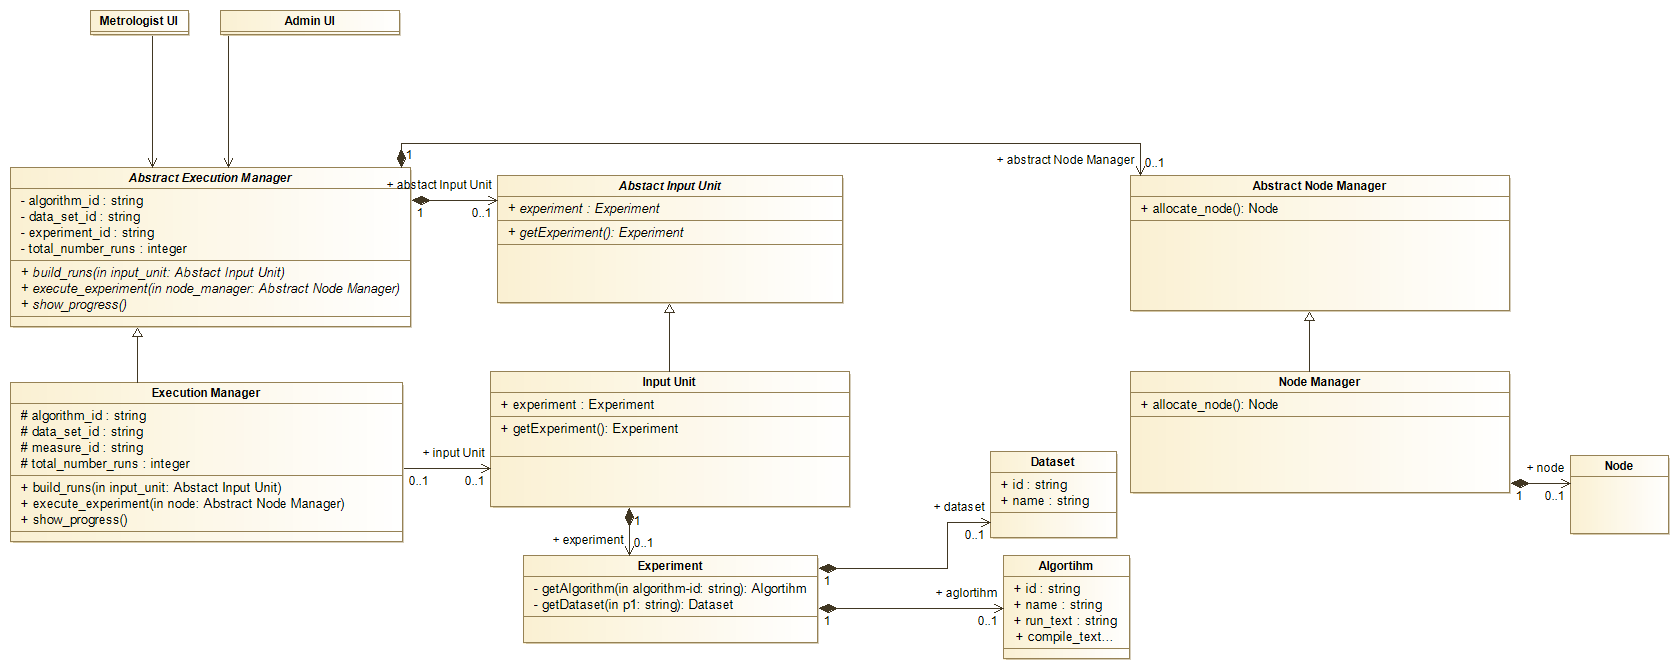
\includegraphics[width=12cm,height=26cm,keepaspectratio]{execution_manager/images/execution_manager_class_diagram.png}
	\begin{center}
	    \small{Figure 1: Class diagram for Execution Manager}
    \end{center}
    
    \par{\textbf{Design Pattern Used} \\ \\
	I used the mediator design pattern because the execution manager uses the input unit as well as the node manager to perform the build runs and execute experiment respectively. The execution manager also persists to the admin UI and the Metrologist UI thus a pattern that can communicate with the reinvent modules and not be extremely dependent is needed. That is why I selected the mediator pattern because it encapsulates the way that objects communicate with each other thus the relevant modules can communicate with each other without knowing the components underlying structure. By using this pattern the modules will be loosely coupled which makes the overall structure of the system much better and easier to manage.In this case the mediator is the \textbf{Execution Manager}  is the Mediator. The \textbf{Input Unit} and \textbf{Node Manager } are the colleagues of the mediator. The \textbf{Metrologist} and \textbf{Admin UI} are the colleagues and as you can see modules are encapsulated.}
		
\subsection{Activity diagram}
    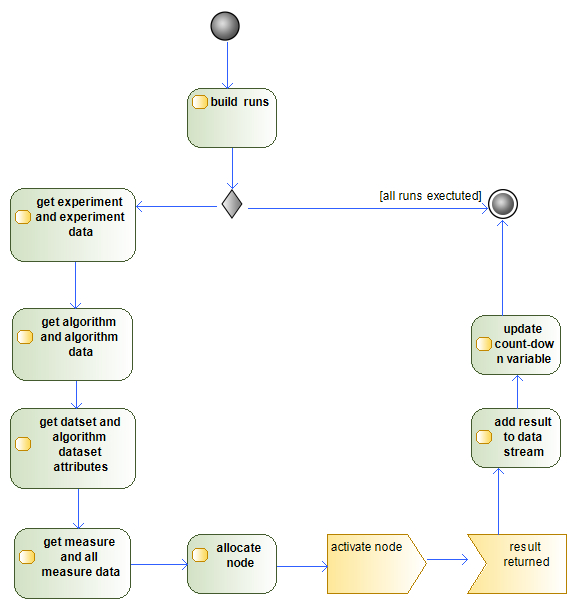
\includegraphics[width=12cm,height=26cm,keepaspectratio]{execution_manager/images/execution_manager_activity_diagram.png}
	\begin{center}
	    \small{Figure 2: Activity diagram for Execution Manager}
    \end{center}


\subsection{Sequence diagram}
    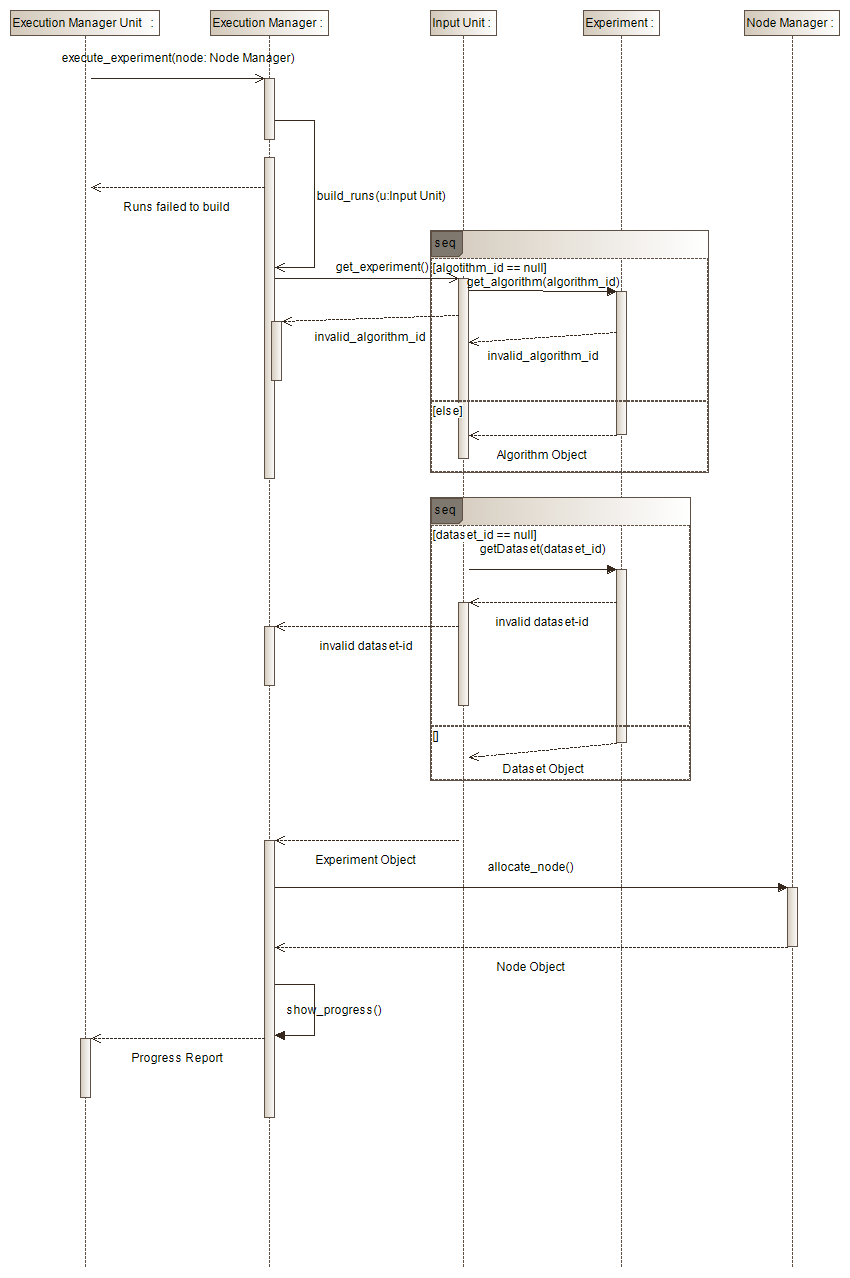
\includegraphics[width=12cm,height=26cm,keepaspectratio]{execution_manager/images/execution_manager_sequence_diagram.png}
	\begin{center}
	    \small{Figure 3: Sequence diagram for Execution Manager}
    \end{center}

\subsection{State diagram}
    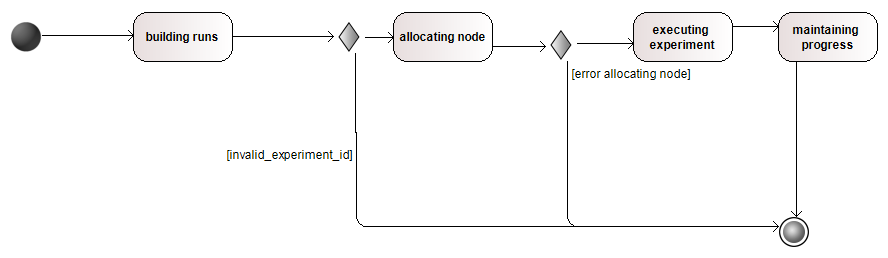
\includegraphics[width=12cm,height=26cm,keepaspectratio]{execution_manager/images/execution_manager_state_diagram.png}
	\begin{center}
	    \small{Figure 4: State diagram for Execution Manager}
    \end{center}




\subsection{Use Case diagram}
    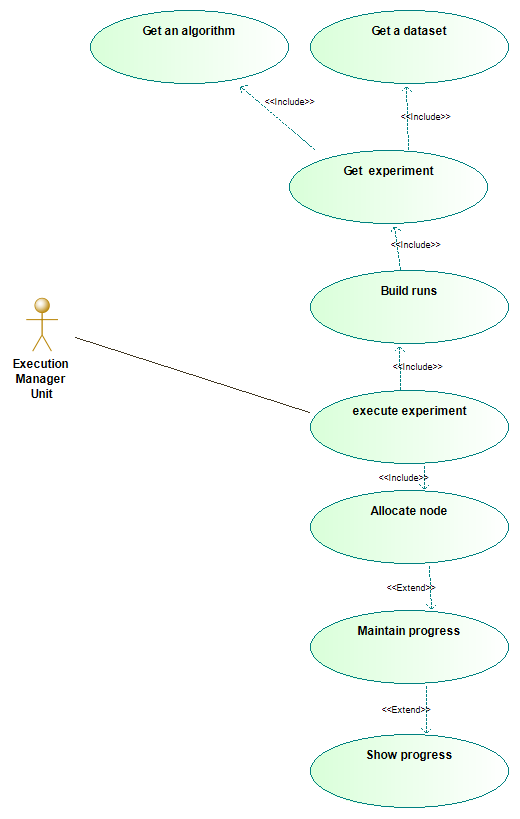
\includegraphics[width=12cm,height=15cm,keepaspectratio]{execution_manager/images/execution_manager_use_case_diagram.png}
    \begin{center}
    	\small{Figure 5: Use case diagram for Execution Manager}
    \end{center}